\hypertarget{backfacing2_8cpp}{
\subsection{/home/luiggi/Documents/Research/Meshless\_\-RBF/NEW/RBFSoft/examples/08BackwardFacingStep/backfacing2.cpp File Reference}
\label{backfacing2_8cpp}\index{/home/luiggi/Documents/Research/Meshless\_\-RBF/NEW/RBFSoft/examples/08BackwardFacingStep/backfacing2.cpp@{/home/luiggi/Documents/Research/Meshless\_\-RBF/NEW/RBFSoft/examples/08BackwardFacingStep/backfacing2.cpp}}
}
Backward-acing Step in 2D.  




\subsubsection{Detailed Description}
Backward-acing Step in 2D. 

In this example the Backward-facing step is solved in the vorticity - stream function formulation. The equations to solve are: \[ \frac{\partial^2 \psi}{\partial x^2} + \frac{\partial^2 \psi}{\partial y^2} = w \] and \[ \frac{\partial^2 w}{\partial x^2} + \frac{\partial^2 w}{\partial y^2} = Re \left( u \frac{\partial w}{\partial x} + v \frac{\partial w}{\partial y} \right) \] where $ \psi $ is the stream function and the vorticity and the velocity are defined as follows \[ (u, v) = (\frac{\partial \psi}{\partial y}, -\frac{\partial \psi}{\partial x}) \\ w = \frac{\partial v}{\partial x} - \frac{\partial u}{\partial y} \] The boundary conditions are the typical for the backward-facing step, see for example \mbox{[}\mbox{]}.  \begin{Image}
\begin{center}
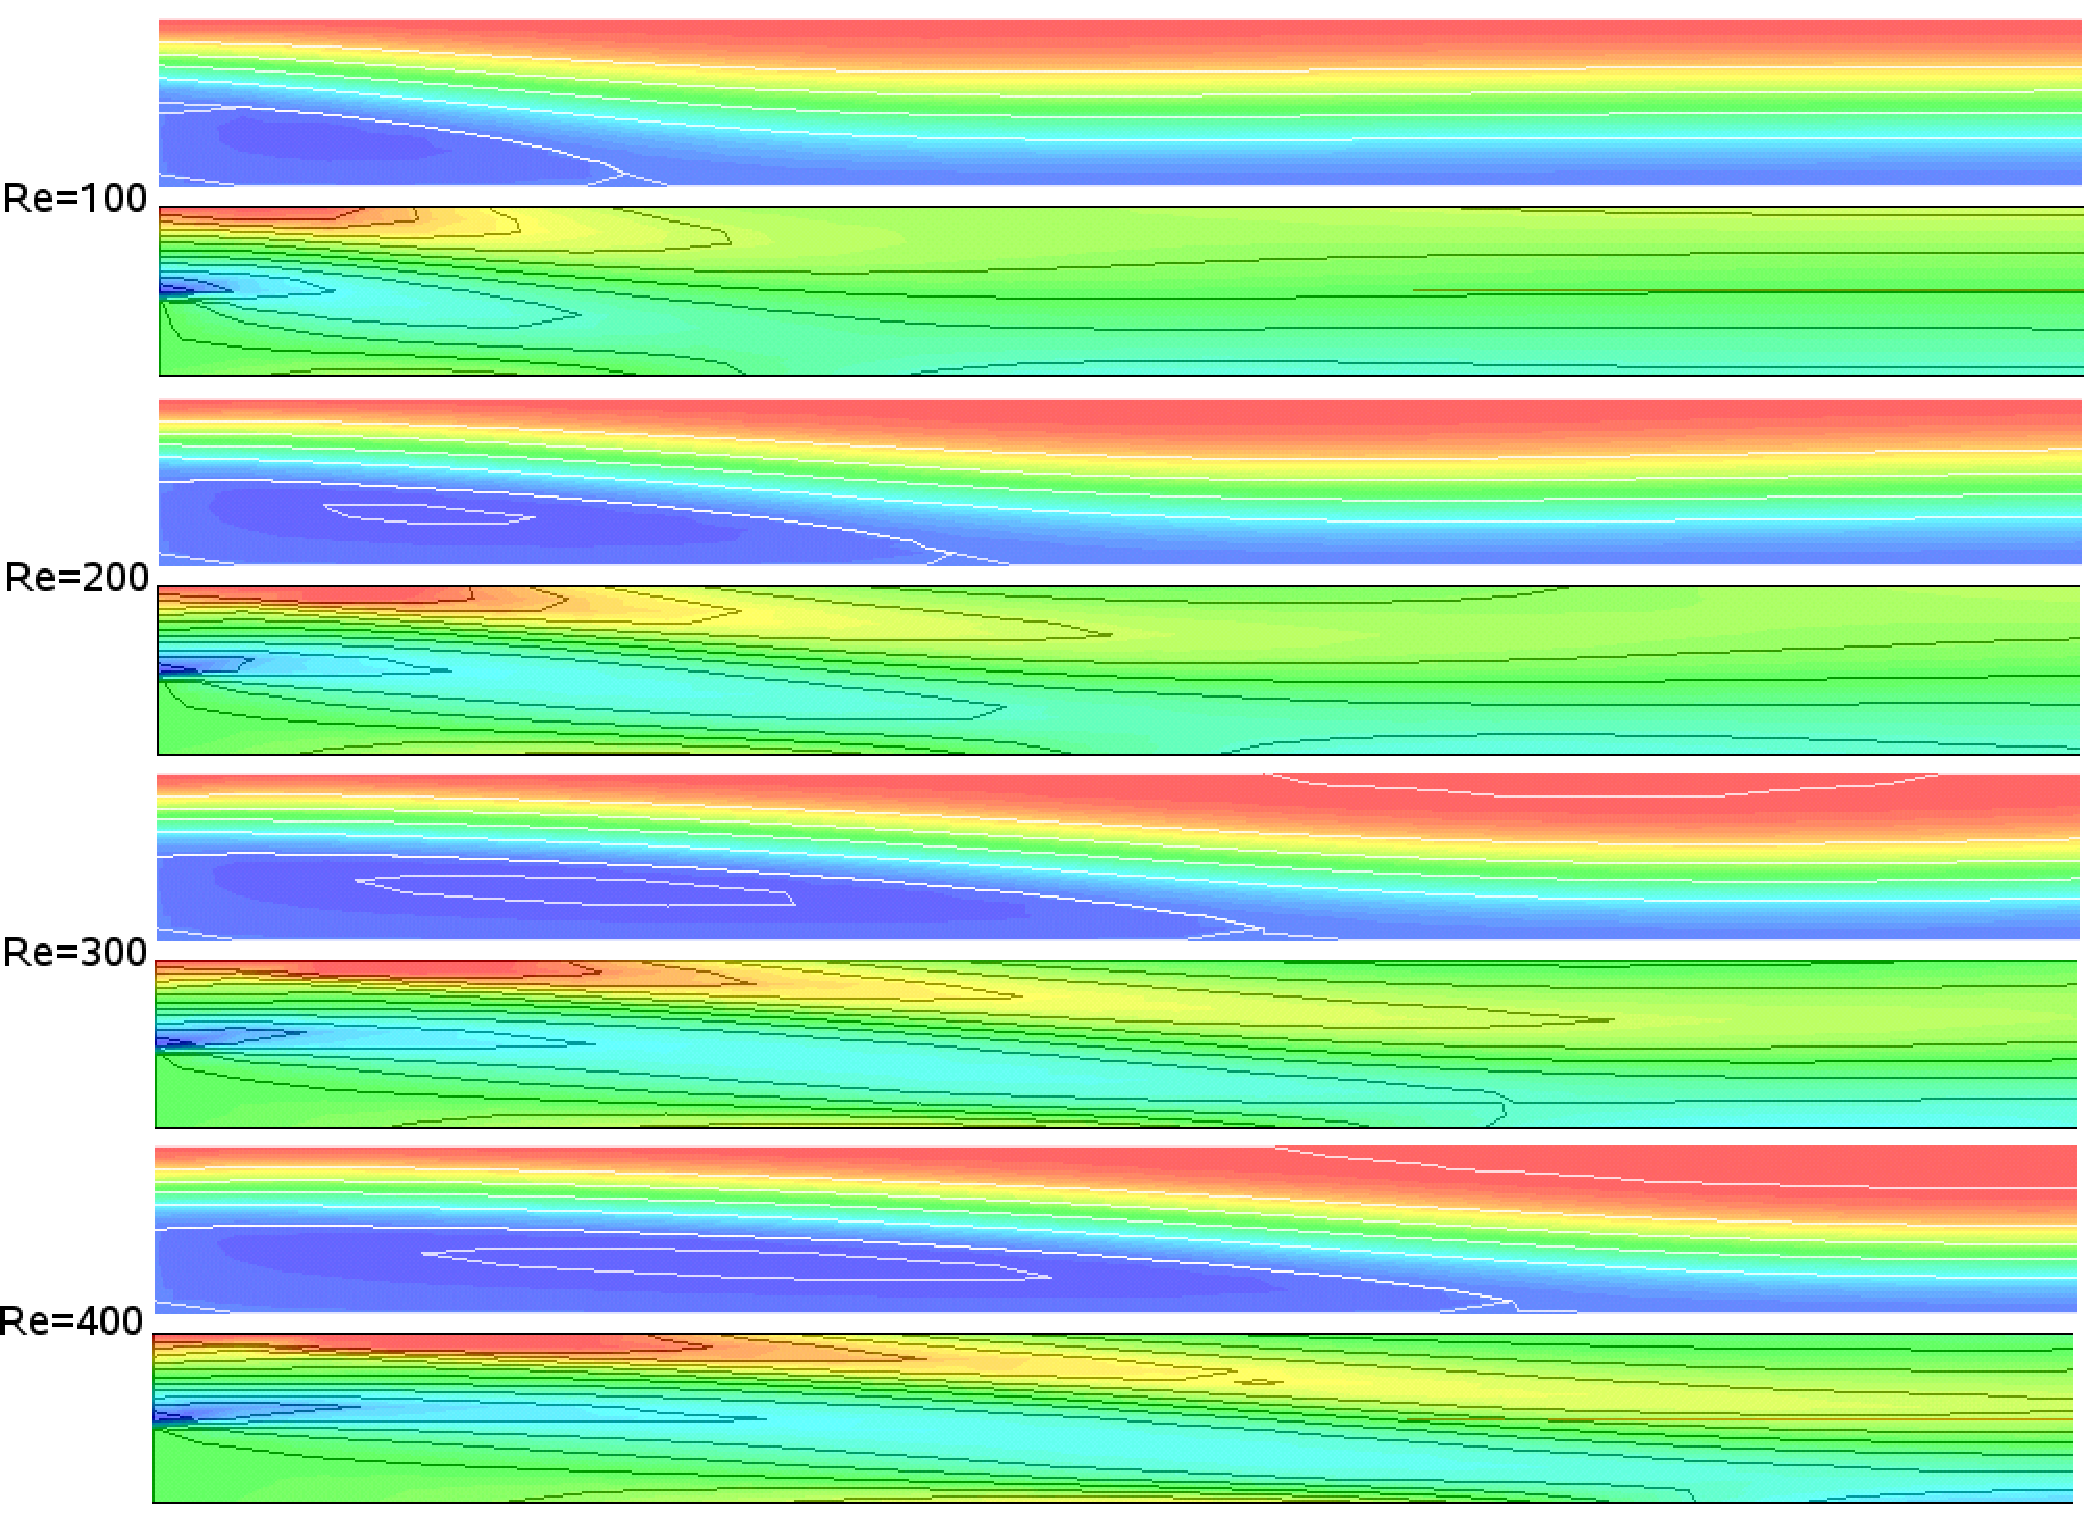
\includegraphics[width=5cm]{solbackfacing}\caption{Streamfunction and Vorticity}
\end{center}
\end{Image}
 \begin{Desc}
\item[Input]The {\tt input} file contains the initial data to setup the problem.\begin{itemize}
\item {\tt hx}, hy, Nx, Ny Size of the cavity and number of points on each axis.\item {\tt rtype}, {\tt ep} point distribution, randomness\item {\tt dt}, {\tt max\_\-iter}, {\tt max\_\-knots} time step, time iterations, neighbors\item {\tt c} shape parameter for MQ-RBF kernel ($c < 0$ implies $ c = 1/\sqrt{N}$).\item {\tt Re} Reydolds number.\item {\tt beta\_\-s}, beta\_\-v, beta\_\-vb under-relaxation parameters for streamfunction, vorticity and boundary conditions for vorticity.\item {\tt gmres\_\-tol}, {\tt tolerance} Tolerance for GMRES, global tolerance\item {\tt scale\_\-x}, scale factor for x-coordinates. \end{itemize}
\end{Desc}
\begin{Desc}
\item[Output]\begin{itemize}
\item {\tt xy\_\-knots.dat} coordinates of random points;\item {\tt solStream.dat} (x,y,u) Streamfunction.\item {\tt solVort.dat} (x,y,u) Vorticity.\end{itemize}
\end{Desc}
\begin{Desc}
\item[Author:]Luis M. de la Cruz Wed \mbox{[} Mon Apr 7 09:58:44 BST 2008 \mbox{]} \end{Desc}


Definition in file \hyperlink{backfacing2_8cpp-source}{backfacing2.cpp}.